\section{Results}
    \subsection{Initial Data Exploration}
        During the initial data exploration, some of the features that were discussed earlier were gathered. Due to the fact that some features are quite complex to retrieve, the initial retrieval did not cover them all. During the later stages of this project, we would like to make all our features visual in some way or another; we found that this gives valuable insights regarding the structuring of the data we are dealing with.
        
        To actually make the data that was gathered more useful, some plots were made. 
        Figures \ref{fig:language-frequency-plot}, \ref{fig:star-distribution-plot}, \ref{fig:number-of-members-per-project-plot} and \ref{fig:number-of-commits-all-plot} are generated from the data that was gathered from the sample.
        An important observation is that almost all the data that was gathered is strongly right skewed. %this makes our life a pain.
        This implies that we might need to normalize it in the future, but that decision is yet to be made. 
        
	    \begin{figure}
	        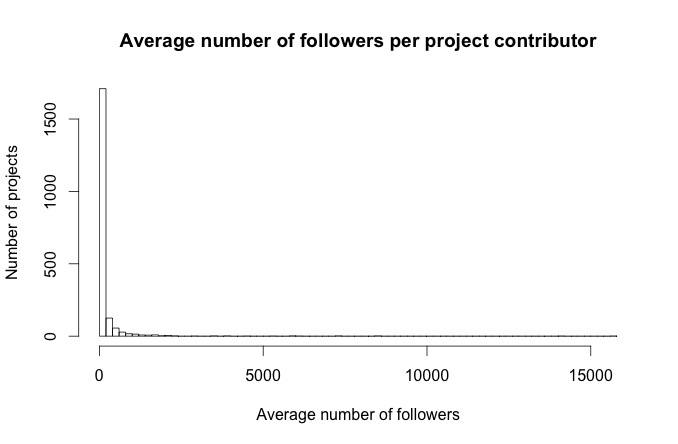
\includegraphics[width=250pt]{figures/average-number-of-followers-per-project-contributor}
	        \caption{The average number of followers per project contributor}
	        \label{fig:avg-follower-contributor-plot}
	    \end{figure}

	    \begin{figure*}
	        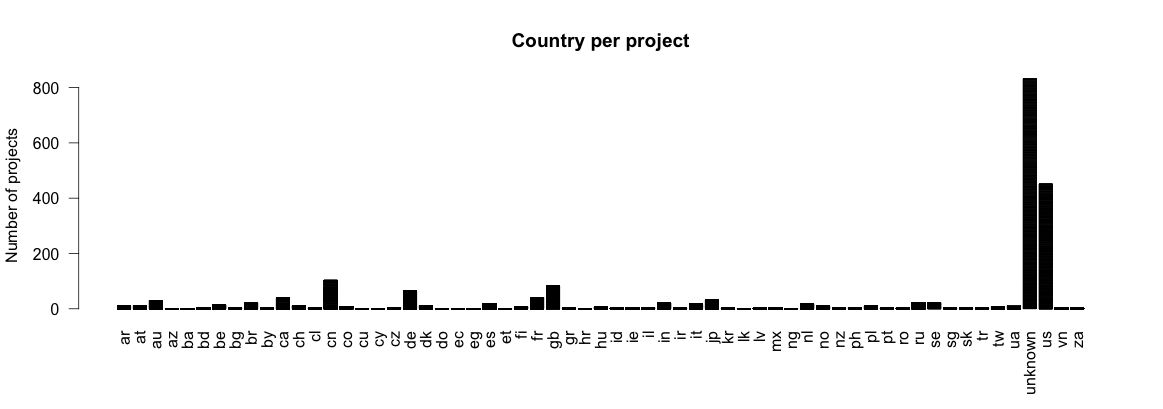
\includegraphics[width=500pt]{figures/country-per-project}
	        \caption{An overview of the countries where the project was created}
	        \label{fig:country-plot}
	    \end{figure*}

	    \begin{figure}
	        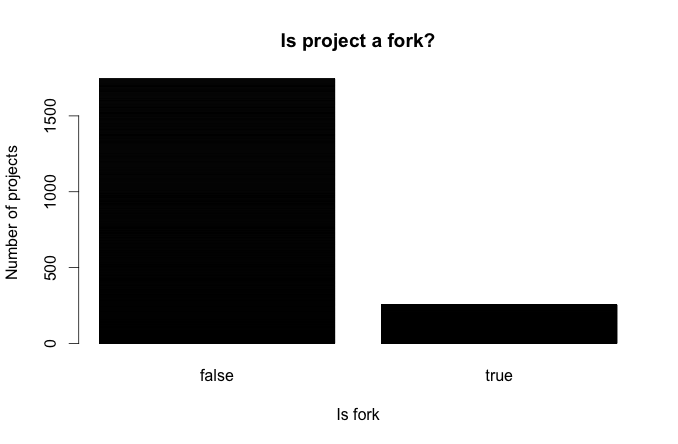
\includegraphics[width=250pt]{figures/isfork-per-project}
	        \caption{A histogram showing whether a project is a fork or not}
	        \label{fig:is-fork-plot}
	    \end{figure}

	    \begin{figure*}
	        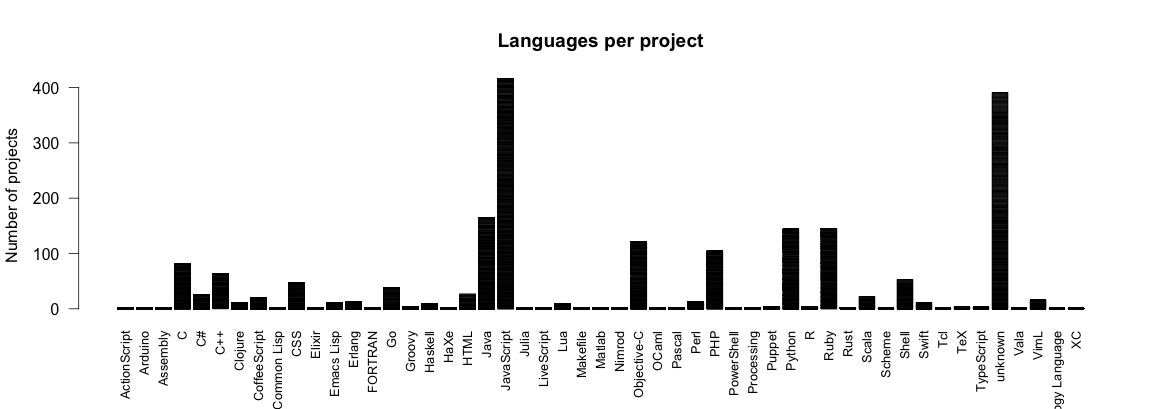
\includegraphics[width=500pt]{figures/languages-per-project}
	        \caption{An overview of the languages user per project}
	        \label{fig:language-frequency-plot}
	    \end{figure*}

	    \begin{figure}
	        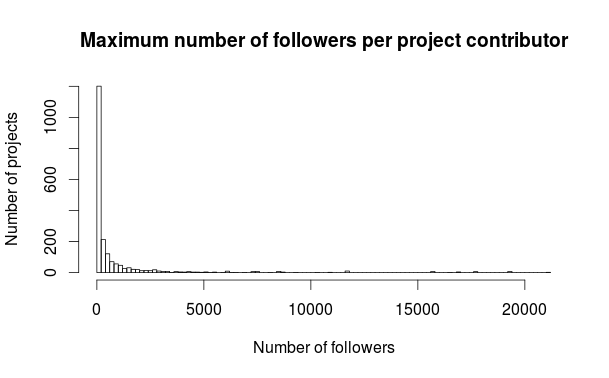
\includegraphics[width=250pt]{figures/maximum-number-of-followers-per-project-contributor}
	        \caption{The maximum number of followers per project contributor}
	        \label{fig:max-follower-contributor-plot}
	    \end{figure}

	    \begin{figure}
	        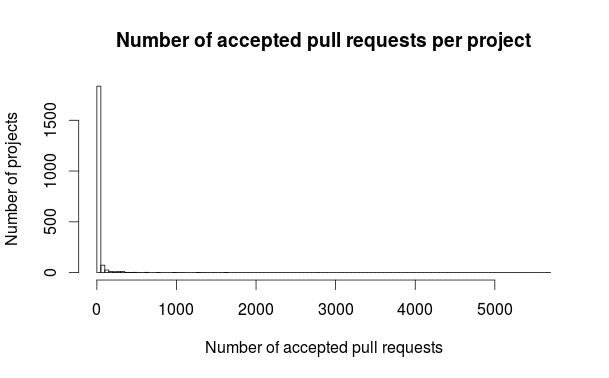
\includegraphics[width=250pt]{figures/nr-of-accepted-pull-requests-per-project}
	        \caption{The number of accepted pull requests per project}
	        \label{fig:accepted-pull-plot}
	    \end{figure}

	    \begin{figure}
	        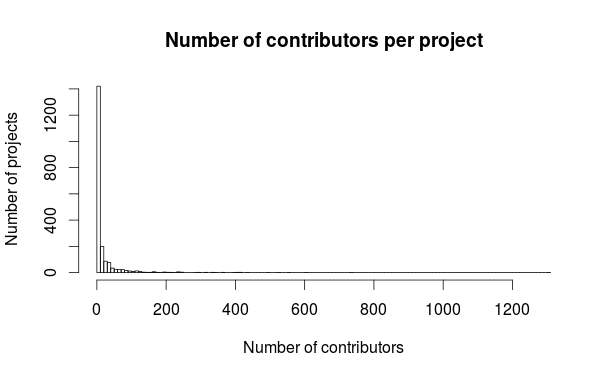
\includegraphics[width=250pt]{figures/nr-of-contributors-per-project}
	        \caption{The number of contributors per project}
	        \label{fig:nr-contributors-plot}
	    \end{figure}

	    \begin{figure}
	        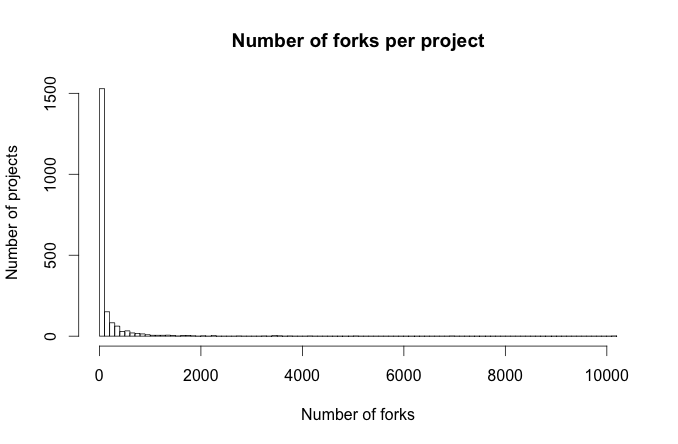
\includegraphics[width=250pt]{figures/number-of-forks-per-project}
	        \caption{The number of forks per project}
	        \label{fig:nr-forks-plot}
	    \end{figure}

	    \begin{figure}
	        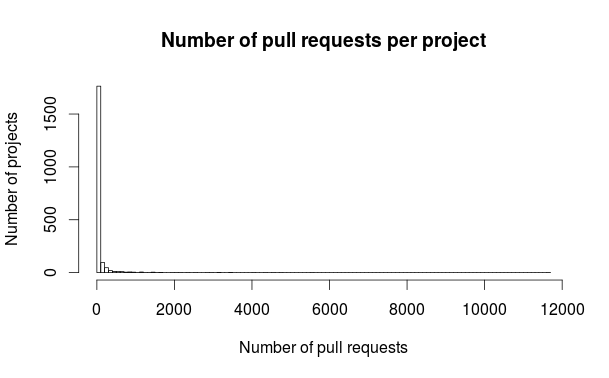
\includegraphics[width=250pt]{figures/number-of-pull-requests-per-project}
	        \caption{The number of pull requests per project}
	        \label{fig:nr-pull-requests-plot}
	    \end{figure}

	    \begin{figure}
	        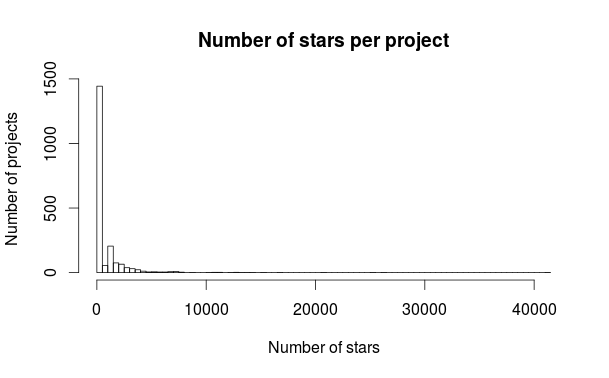
\includegraphics[width=250pt]{figures/number-of-stars-per-project}
	        \caption{The number of stars per project}
	        \label{fig:nr-stars-plot}
	    \end{figure}

	    \begin{figure}
	        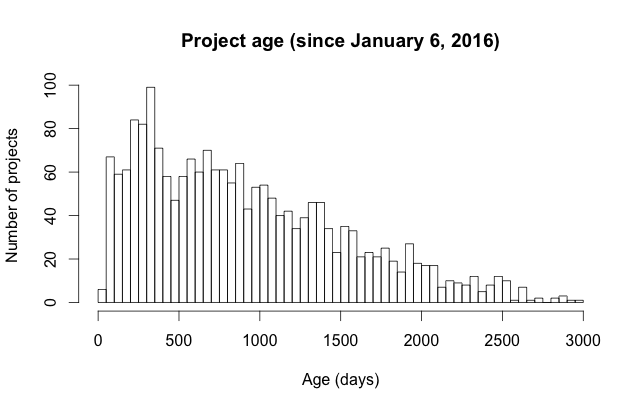
\includegraphics[width=250pt]{figures/project-age}
	        \caption{The age of the project in days from January 6, 2016}
	        \label{fig:age-plot}
	    \end{figure}

	    \begin{figure}
	        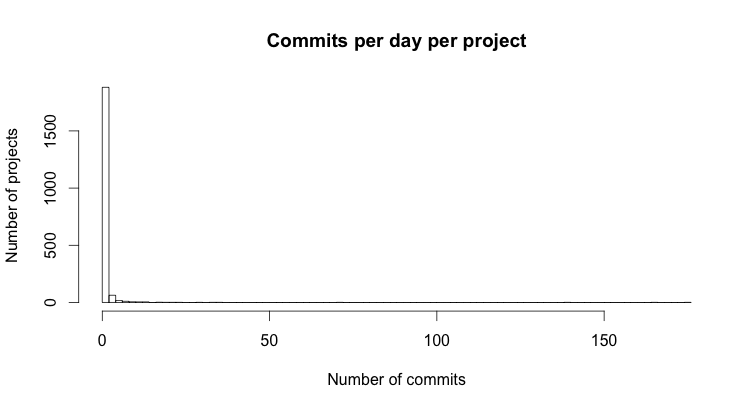
\includegraphics[width=250pt]{figures/commits-per-day-per-project}
	        \caption{The number of commits per day per project}
	        \label{fig:nr-commits-day-plot}
	    \end{figure}

	    \begin{figure}
	        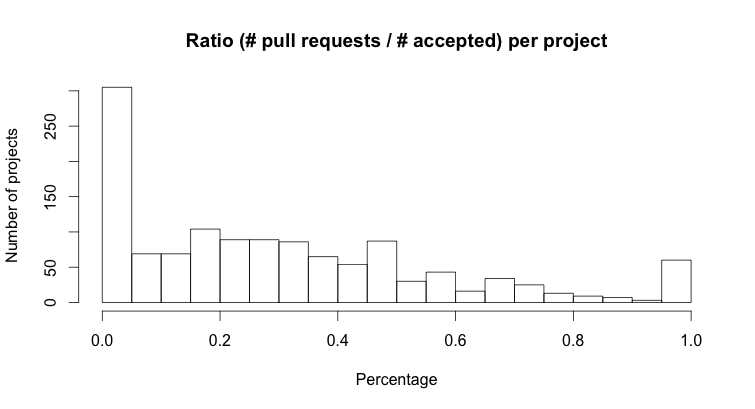
\includegraphics[width=250pt]{figures/ratio-pull-request-per-project}
	        \caption{The ratio of accepted pull requests per project}
	        \label{fig:ratio-pull-requests-plot}
	    \end{figure}

    
    \subsection{Testing the model}
        \todo{Will be added later on}
